%\documentclass[12pt]{article}
%\documentclass[a4paper, 12pt]{scrartcl}
%\voffset=-0.9in
%\hoffset=-0.6in
\documentclass[DIV=12]{article}
\setlength{\textheight}{9.1in}
\setlength{\textwidth}{7in} 
\usepackage[margin=1.1in]{geometry}
%\usepackage[justification=justified,singlelinecheck=off]{caption}

\newcommand{\pubSpace}{\vspace{-0.3in}}
\newcommand{\confSpace}{\vspace{-0.24in}}
\newcommand{\respSpace}{\vspace{-0.2in}}
\newcommand{\COffset}{C_{\mathrm{offset}}} 
\newcommand{\rhoOffset}{\rho_{\mathrm{offset}}}
\newcommand{\CPyr}{C^{\mathrm{pyr}}}

%\cofoot{\footnotesize{\rm{Pascal Grange (August 2013)}} {\rm{\ttfamily{ pascal.grange@polytechnique.org}}}}


\let\oldbibliography\thebibliography
\renewcommand{\thebibliography}[1]{%
  \oldbibliography{#1}%
  \setlength{\itemsep}{-1pt}%
{\small
\bibliography{bibfile}}
}


\usepackage[dvips]{color}
\bibliographystyle{plain}

\usepackage{graphicx}
%\usepackage{pdfpages}
%\usepackage{multicol}
%\usepackage{pstricks,pst-grad}
%\usepackage{epsfig}
\usepackage{amsmath}

%\usepackage{subfig}
%\usepackage{tikz}
%\usepackage{verbatim}
\usepackage{amsmath}

%\usepackage{array}
%\pagestyle{scrheadings}

\newcommand{\voxel}{{\mathrm{voxel}}}
\newcommand{\gene}{{\mathrm{gene}}} 
\newcommand{\type}{{\mathrm{type}}}
\newcommand{\widthCoeff}{0.8}
\newcommand{\visibleGreen}{green!50!black}

\newcommand{\eBase}{(\vec{e_1}, \vec{e_2},\vec{e_3})}
\newcommand{\eBasePrime}{\left(\vec{e'_1}, \vec{e'_2},\vec{e'_3}\right)}
\newcommand{\maxX}{12}
\newcommand{\maxY}{12}

%\newcolumntype{S}{>{\centering\arraybackslash} m{\widthCoeff\linewidth} }

%\cofoot{\footnotesize{\rm{XJTLU, MTH308, 2014)}}}
%\title{\Huge{Research statement}\\
%    \vspace{3mm}
%       \Large{Computational biology: data analysis tools in high dimensions}}
%\author{Pascal Grange}
%\date{}
\begin{document}
%\maketitle
%\begin{flushleft}
%\Large{\bf{Research statement: data analysis tools for computational biology in high dimensions}}\\
%\large{\bf{Pascal Grange}}
%\end{flushleft}\textsc{\LARGE University of Beer}\\[1.5cm]

%\textsc{\Large Final year project}\\[0.5cm]

% Title
\title{
\noindent\hrulefill
\begin{flushleft}
{\Large \bf{XJTLU, MTH308 (Cartesian tensors and mathematical models of (elastic) solids and viscous fluids), Semester 2, 2015\\
\vspace{8mm}
\hrule
\vspace{6mm}
 Lecture 2, 10th March, 2015: Kinematics and deformations}}
\vspace{8mm}
\hrule
\vspace{6mm}
{\Large{Pascal Grange\\
Department of mathematical sciences\\
{\ttfamily{pascal.grange@xjtlu.edu.cn}}\\
}}
\noindent\hrulefill
\end{flushleft}}
\date{}
\author{}
\maketitle
%\noindent\hrulefill
\vspace{-3mm}

{\bf{Keywords.}} Kinematics, flows, tangent vectors (transformation of line elements, deformation, differential geometry).\\

\vspace{3mm}

{\bf{Convention.}} Unless otherwise stated, the sum rule over repeated indices is observed.\\


\tableofcontents

\vspace{12mm}
In this chapter we will develop the mathematical the description  of 
 movements of continuous media  (which can be elastic solids or fluids) without studying their causes. This is the kinematics of 
 continuous media. A function of {\emph{initial position and time}} is
 used to describe the motion (or {\emph{flow}}) of the continuous medium. 
 To decide whether the medium is deformed, we have to compute how
 scalar products of vectors change under the flow (see Fig. \ref{figur} for
 a physical example on a solid: we are going to describe mathematically how the grid 
on the l.h.s. of the figure is deformed).\\
Technically, the first chapter was entirely based on linear algebra (we learned how the components
 of a fixed object such as a vector or the matrix of a linear application transform under a change of base). 
 This chapter will be mostly based on differential geometry: we will work with a 
 fixed base, but study the tangent vectors to moving curves.


\section{Lagrangian description of flows}
\subsection{Definitions and notations}
To avoid boundary effects, let us study a sample of continuous 
medium (solid or fluid) that "fills the entire space" (meaning we are describing
matter at scales that are large compared to the size of molecules, but we are far away from 
 the boundaries of the sample).\\

The space ${\mathbf{R}}^3$ is endowed with 
 an orthonormal base $(\vec{e_1}, \vec{e_2}, \vec{e_3})$ (which will be kept fixed in this chapter)
  and a
 fixed origin $O$, so the position of a material point $M$ can be described 
 by its coordinates, $\overrightarrow{OM} =\vec{x}= x_i\vec{e_i}$.
We are interested in the way  classical particles (small lumps of continuous medium, which could be 
visualized using tracers in a fluid, or simply by marking the surface by a grid on a solid, as in Fig. \ref{figur}) move over time. Let us say that a particle
 is at position $\vec{X}$ at time $t =0$ (one says that $\vec{X}$ is the initial position of the particle). 
 Let us say we are interested in the deformation of the medium between time $t=0$ and some final time $T$ (the duration
 of an experiment for instance). \\
 
 The position of a material particle at time $t >0$
 can be described by a vector which depends on $t$ and on the initial position.
 Let us denote this vector by $\Phi_1(\vec{X}, t) \vec{e_1} + \Phi_2( \vec{X},t)\vec{e_2} + \Phi_3( \vec{X}, t )\vec{e_3}$.
 Since we can consider any initial position $\vec{X}$, we have just defined an application $\vec{\Phi}$
 that describes the movements of the continuous medium over a time between $t=0$ and $t=T$:

\begin{equation}
 {\mathbf{R}^3}\times [ 0, T] \longrightarrow {\mathbf{R}^3}
\end{equation}
\begin{equation}
 (\vec{X},t)\mapsto \vec{\Phi}( \overrightarrow{X},t) = \Phi_1(\vec{X}, t) \vec{e_1} + \Phi_2( \vec{X},t) \vec{e_2} + \Phi_3( \vec{X}, t ) \vec{e_3}.
\label{flowDef}
\end{equation}

\begin{figure}[htp]
 \centering

  \begin{tabular}{cc}

    % Requires \usepackage{graphicx}

    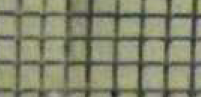
\includegraphics[width=60mm]{recGrid.png}&

    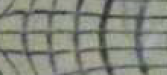
\includegraphics[width=60mm]{recGridPrime.png}\\
  \end{tabular}
\label{figur}\caption{A sample of perspex with 
 orthogonal lines drawn with a pen at $t=0$, and at at some time $t>0$ after traction.}

\end{figure}
We will assume that the application $\vec{\Phi}$ is continuous (and has as many continuous derivatives as we need) in 
 all the variables, as we want to study smooth deformations. Continuity w.r.t.  time at time $t=0$ implies 
 that for all $\vec{X}$ in $\mathbf{R}^3$, we have the property $\vec{\Phi}(\vec{X},0) = \vec{X}.$\\

We want to ask the following question (explicit examples will be given in the exercises): {\bf{given the application $\vec{\Phi}$}},
  and two vectors in the initial state, {\emph{can we compute the evolution of the scalar product of these two vectors?}}


\subsection{Computing the tangent to a curve in three dimensions}
 $\bullet$ {\bf{Let us parametrize a straigth line at time $t=0$.}}
 With the system of coordinates described by the origin $O$ and the base  $(\vec{e_1}, \vec{e_2}, \vec{e_3})$, 
 consider the particle which is at position $\vec{X}= \vec{OM}$ in the continuous medium, at time $t=0$.
 We can move around this vector by adding some vector $\vec{h}\in \mathbf{R}^3$ to it.
 We will need  to do differential calculus (in order to compute tangent vectors), so let us introduce a scalar parameter
 $s\in \mathbf{R}$, which we will eventually let go to 0.\\

If we consider the set of all possible values of the parameter $s$, we get the straight 
 line going through the point $M$ in direction $\vec{h}$. 
The vector $\vec{h}$ is the tangent vector of the straight line that
 goes through $M$ in direction $\vec{h}$, as we have
\begin{equation}
 \frac{1}{s}\left( (\vec{X}+ s\vec{h} ) - \vec{X}\right)\longrightarrow_{s\rightarrow 0} \vec{h}.
 \label{tangentFirst}
\end{equation}
{\bf{NB:}} {\bf{the parameter $s$ is not time, it is just a geometric parameter describing 
 a straight line at a fixed time ($t=0$).}}\\

 $\bullet$ {\bf{ What happens to this line through time? It is mapped to a line defined through $\vec{\Phi}$.}}
 What does this situation look like at time $t>0$?\\
By definition of the flow, the  particle that was at $\vec{X}$ 
 is now at $\vec{\Phi}(\vec{X},t)$ and the particle that was at $\vec{X}+ s\vec{h}$ 
 is now at $\vec{\Phi}(\vec{X}+ s\vec{h},t)$, 
 so the quantity we studied in Eq. \ref{tangentFirst}
 has now become
\begin{equation}
 \frac{1}{s}\left( \vec{\Phi}(\vec{X}+ s\vec{h},t) -  \vec{\Phi}(\vec{X},t) \right)
 \label{accrFinal}
\end{equation}
 Let us study its limit when $s$ goes to zero, which is\footnote{As an exercise, the 
 reader should put the symbols $\vec{X}, \vec{h}, \vec{\Phi}(\vec{X},t),\vec{\Phi}(\vec{X}+\vec{h},t)$ on Fig. \ref{figur}, and draw the two curves we 
 are talking about.}  the tangent 
 to the curve $s \in \mathbf{R} \mapsto   \vec{\Phi}(\vec{X}+ s\vec{h},t)$.\\
 

Let us write all the components in matrix form in the base $\eBase$
to compute this tangent:
\begin{equation}
\vec{\Phi}(\vec{X}+ s\vec{h},t) -  \vec{\Phi}(\vec{X},t) =   \left(
   \begin{array}{l}
       \Phi_1(\vec{X}+ s\vec{h},t) - \Phi_1(\vec{X},t)\\
      \Phi_2(\vec{X}+ s\vec{h},t) - \Phi_2(\vec{X},t)  \\
       \Phi_3(\vec{X}+ s\vec{h},t) - \Phi_3(\vec{X},t)\\
   \end{array}
   \right)
\label{accrVector}
\end{equation}

Let us assume that the components of $\vec{\Phi}$ are smooth functions (they posess
derivatives at all orders). One can write a first-order Taylor expansion 
 of each of the  components of the vector in Eq. \ref{accrVector}. For example:
\begin{equation}
 \Phi_1(\vec{X}+ s\vec{h},t)  = \Phi_1(\vec{X},t) + s h_1 \frac{\partial\Phi_1}{\partial X_1}(\vec{X},t) + s h_2 \frac{\partial\Phi_1}{\partial X_2}(\vec{X},t)+
   s h_3 \frac{\partial\Phi_1}{\partial X_3}(\vec{X},t) + o(s).
\end{equation}
Hence the quantity 
\begin{equation}
 \frac{1}{s}\left(\Phi_1(\vec{X}+ s\vec{h},t)  - \Phi_1(\vec{X},t) \right) =  h_1 \frac{\partial\Phi_1}{\partial X_1}(\vec{X},t) +  h_2 \frac{\partial\Phi_1}{\partial X_2}(\vec{X},t)+
   h_3 \frac{\partial\Phi_1}{\partial X_3}(\vec{X},t) + \frac{o(s)}{s},
\end{equation}
 and its limit when $s$ goes to zero is given by:
\begin{equation}
h_i \frac{\partial \Phi_1( \vec{X})}{\partial X_i},
\end{equation}
 where the sum rule over doubled indices is applied.
 The computation can be repeated for $\Phi_2$ and $\Phi_3$, and one obtains the following limit:
\begin{equation}
\frac{1}{s}\left(
\vec{\Phi}(\vec{X}+ s\vec{h},t) -  \vec{\Phi}(\vec{X},t)\right) \longrightarrow_{s\rightarrow 0}   \left(
   \begin{array}{l}
      h_i \frac{\partial \Phi_1( \vec{X},t)}{\partial X_i}\\
     h_i \frac{\partial \Phi_2( \vec{X},t)}{\partial X_i}\\
     h_i \frac{\partial \Phi_3( \vec{X},t)}{\partial X_i}
   \end{array}
 \right).
\end{equation}


$\bullet$ {\bf{A line is mapped to a line, tangent vectors are mapped to tangent vectors.}}
 Hence the vector $\vec{h} = h_j\vec{e_j}$pointing from $\vec{X}$ is mapped to 
 the vector 
\begin{equation}
h_i \frac{\partial \Phi_j( \vec{X})}{\partial X_i} \vec{e_j} = h_i T_{ji} (\vec{X},t) \vec{e_j},
\label{transportVec}
\end{equation}
 by the flow, where we have defined 
 the matrix $T$ (whose value depends on the initial position $\vec{X}$ by:\\
\begin{equation}
 T_{ij} (\vec{X},t)=  \frac{\partial \Phi_i( \vec{X},t)} {\partial X_j},
 \label{equation}
\end{equation}
which maps vectors from position $\vec{X}$ to position $\vec{\Phi}(\vec{X},t)$.
 $T$ is called the {\emph{strain tensor}}. It depends on the initial point $\vec{X}$ 
 so one could (should) call it {\emph{strain tensor field}}.
%}

\section{How does the scalar product change under the flow?}

 Taking a pair of vectors $\vec{h} = h_i\vec{e_i}$ and $\vec{u} = u_i \vec{e_i}$
 starting from position $\vec{X}$, one can transport both vectors by the flow
 using Eq. \ref{transportVec}, and compute the dot-product of the resulting vectors:\\
\begin{equation}
\large{
   \begin{array}{ll}
 \left( h_i \frac{\partial \Phi_j( \vec{X},t)}{\partial X_i} \vec{e_j} \right) .\left( u_k \frac{\partial \Phi_l( \vec{X},t)}{\partial X_k} \vec{e_l}\right) &= h_i u_k\frac{\partial \Phi_j( \vec{X},t)}{\partial X_i}\frac{\partial \Phi_l( \vec{X},t)}{\partial X_k}\delta_{jl} \\
 &=  h_i u_k\frac{\partial \Phi_j( \vec{X},t)} {\partial X_i}\frac{\partial \Phi_j( \vec{X},t)}{\partial X_k}\\
& =  h_i u_k  T_{ji}(\vec{X},t) T_{jk}(\vec{X},t).
\end{array}}
\label{dotTransform}
\end{equation}


 One could be tempted to say that there is "no deformation" if the matrix $T$ is the identity matrix. However this
condition is too restrictive. Indeed we can see from Eq. \ref{dotTransform}
 that if $T_{ji}T_{jk} = \delta_{ik}$, the scalar product is preserved (hence the grid drawn on Fig. \ref{figur}
 is not deformed, just transported). Hence we see that the local deformations
 are measured by the measured by the difference $T_{ji}T_{jk} - \delta_{ik}$.


\end{document}

 






 






